\section[Introduction]{Introduction}
\label{sec:introduction}

\begin{frame}{Bifurcations and Critical Slowing Down}
	\textbf{Bifurcation}: A qualitative change in the `motion' of a dynamical System due to a quantitative change in one of its parameters. Serious bifurcations, called \textcolor{red}{Critical Bifurcations}, cause the system to become unstable from stable.
\end{frame}

\begin{frame}{Bifurcations and Critical Slowing Down}
	\begin{figure}
		\centering
		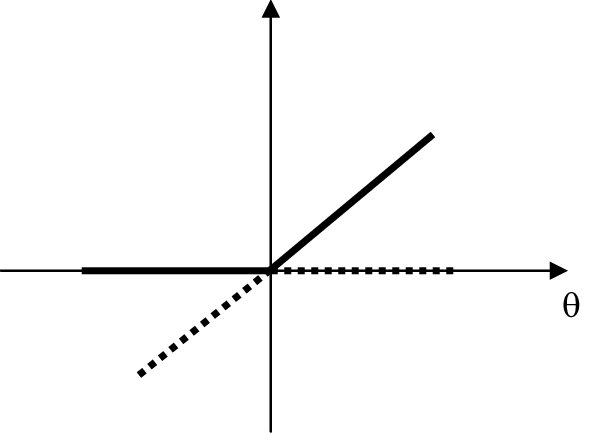
\includegraphics[scale=1.00]{../figures/transcriticalBifurcation}
		\label{fig:transcritBifurcation}
		\caption{Bifurcation Diagram showing the Normal form of Transcritical Bifurcation}
		\begin{equation}
		\frac{dx}{dt} = \theta x - x^2
		\end{equation}
	\end{figure}
\end{frame}

\begin{frame}{Bifurcations and Critical Slowing Down}
	\textbf{Critical Slowing Down}: Dynamical Systems exhibit early statistical warning signs before collapsing:
	
	\begin{itemize}
		\item Increased recovery times from perturbations.
		\item Increased signal variance from the mean trajectory.
		\item Increased flicker and asymmetry in the signal
	\end{itemize}

The above three properties can be identified by increasing variance and autocorrelation in time-series measurements taken from the system.
\end{frame}
